\documentclass[a4paper]{article}

\usepackage{inputenc}
\usepackage[british,UKenglish]{babel}
\usepackage{amsmath}
%\usepackage{titlesec}
\usepackage{color}
\usepackage{graphicx}
\usepackage{fancyref}
\usepackage{hyperref}
\usepackage{float}
\usepackage{scrextend}
\usepackage{setspace}
\usepackage{xargs}
\usepackage{multicol}
\usepackage{nameref}

\usepackage{sectsty}
\usepackage{multicol}
\usepackage{multirow}
\usepackage[procnames]{listings}
\usepackage{appendix}

\newcommand\tab[1][1cm]{\hspace*{#1}}
\hypersetup{colorlinks=true, linkcolor=black}
\interfootnotelinepenalty=10000

\newcommand{\cleancode}[1]{\begin{addmargin}[3em]{3em}\texttt{\textcolor{cleanOrange}{#1}}\end{addmargin}}
\newcommand{\cleanstyle}[1]{\text{\textcolor{cleanOrange}{\texttt{#1}}}}


\usepackage[colorinlistoftodos,prependcaption,textsize=footnotesize]{todonotes}
\newcommandx{\commred}[2][1=]{\textcolor{Red}
{\todo[linecolor=red,backgroundcolor=red!25,bordercolor=red,#1]{#2}}}
\newcommandx{\commblue}[2][1=]{\textcolor{Blue}
{\todo[linecolor=blue,backgroundcolor=blue!25,bordercolor=blue,#1]{#2}}}
\newcommandx{\commgreen}[2][1=]{\textcolor{OliveGreen}{\todo[linecolor=OliveGreen,backgroundcolor=OliveGreen!25,bordercolor=OliveGreen,#1]{#2}}}
\newcommandx{\commpurp}[2][1=]{\textcolor{Plum}{\todo[linecolor=Plum,backgroundcolor=Plum!25,bordercolor=Plum,#1]{#2}}}

\def\code#1{{\tt #1}}

\def\note#1{\noindent{\bf [Note: #1]}}

\makeatletter
%% The "\@seccntformat" command is an auxiliary command
%% (see pp. 26f. of 'The LaTeX Companion,' 2nd. ed.)
\def\@seccntformat#1{\@ifundefined{#1@cntformat}%
   {\csname the#1\endcsname\quad}  % default
   {\csname #1@cntformat\endcsname}% enable individual control
}
\let\oldappendix\appendix %% save current definition of \appendix
\renewcommand\appendix{%
    \oldappendix
    \newcommand{\section@cntformat}{\appendixname~\thesection\quad}
}
\makeatother


% "define" Scala
\usepackage[T1]{fontenc}  
\usepackage[scaled=0.82]{beramono}  
\usepackage{microtype} 

\sbox0{\small\ttfamily A}
\edef\mybasewidth{\the\wd0 }

\lstdefinelanguage{scala}{
  morekeywords={abstract,case,catch,class,def,%
    do,else,extends,false,final,finally,%
    for,if,implicit,import,match,mixin,%
    new,null,object,override,package,%
    private,protected,requires,return,sealed,%
    super,this,throw,trait,true,try,%
    type,val,var,while,with,yield},
  sensitive=true,
  morecomment=[l]{//},
  morecomment=[n]{/*}{*/},
  morestring=[b]",
  morestring=[b]',
  morestring=[b]"""
}

\usepackage{color}
\definecolor{dkgreen}{rgb}{0,0.6,0}
\definecolor{gray}{rgb}{0.5,0.5,0.5}
\definecolor{mauve}{rgb}{0.58,0,0.82}

% Default settings for code listings
\lstset{frame=tb,
  language=scala,
  aboveskip=3mm,
  belowskip=3mm,
  showstringspaces=false,
  columns=fixed, % basewidth=\mybasewidth,
  basicstyle={\small\ttfamily},
  numbers=none,
  numberstyle=\footnotesize\color{gray},
  % identifierstyle=\color{red},
  keywordstyle=\color{blue},
  commentstyle=\color{dkgreen},
  stringstyle=\color{mauve},
  frame=single,
  breaklines=true,
  breakatwhitespace=true,
  procnamekeys={def, val, var, class, trait, object, extends},
  procnamestyle=\ttfamily\color{red},
  tabsize=2
}

\lstnewenvironment{scala}[1][]
{\lstset{language=scala,#1}}
{}
\lstnewenvironment{cpp}[1][]
{\lstset{language=C++,#1}}
{}
\lstnewenvironment{bash}[1][]
{\lstset{language=bash,#1}}
{}
\lstnewenvironment{verilog}[1][]
{\lstset{language=verilog,#1}}
{}



%代码段设置
\lstset{numbers=left,
basicstyle=\tiny,
numberstyle=\tiny,
keywordstyle=\color{blue!70},
commentstyle=\color{red!50!green!50!blue!50},
frame=single, rulesepcolor=\color{red!20!green!20!blue!20},
escapeinside=``
}

\graphicspath{ {figures/} }
\usepackage{ctex}
\setCJKmainfont[ItalicFont=Noto Sans CJK SC Bold, BoldFont=Noto Serif CJK SC Black]{Noto Serif CJK SC}
\usepackage{graphicx}
\usepackage{color,framed}%文本框
\usepackage{listings}
\usepackage{caption}
\usepackage{amssymb}
\usepackage{enumerate}
\usepackage{xcolor}
\usepackage{bm} 
\usepackage{lastpage}%获得总页数
\usepackage{fancyhdr}
\usepackage{tabularx}  
\usepackage{geometry}
\usepackage{minted}
\usepackage{graphics}
\usepackage{subfigure}
\usepackage{float}
\usepackage{pdfpages}
\usepackage{pgfplots}
\pgfplotsset{width=10cm,compat=1.9}
\usepackage{multirow}
\usepackage{footnote}
\usepackage{booktabs}

%-----------------------伪代码------------------
\usepackage{algorithm}  
\usepackage{algorithmicx}  
\usepackage{algpseudocode}  
\floatname{algorithm}{Algorithm}  
\renewcommand{\algorithmicrequire}{\textbf{Input:}}  
\renewcommand{\algorithmicensure}{\textbf{Output:}} 
\usepackage{lipsum}  
\makeatletter
\newenvironment{breakablealgorithm}
  {% \begin{breakablealgorithm}
  \begin{center}
     \refstepcounter{algorithm}% New algorithm
     \hrule height.8pt depth0pt \kern2pt% \@fs@pre for \@fs@ruled
     \renewcommand{\caption}[2][\relax]{% Make a new \caption
      {\raggedright\textbf{\ALG@name~\thealgorithm} ##2\par}%
      \ifx\relax##1\relax % #1 is \relax
         \addcontentsline{loa}{algorithm}{\protect\numberline{\thealgorithm}##2}%
      \else % #1 is not \relax
         \addcontentsline{loa}{algorithm}{\protect\numberline{\thealgorithm}##1}%
      \fi
      \kern2pt\hrule\kern2pt
     }
  }{% \end{breakablealgorithm}
     \kern2pt\hrule\relax% \@fs@post for \@fs@ruled
  \end{center}
  }
\makeatother
%------------------------代码-------------------
\usepackage{xcolor} 
\usepackage{listings} 
\lstset{ 
breaklines,%自动换行
basicstyle=\small,
escapeinside=``,
keywordstyle=\color{ blue!70} \bfseries,
commentstyle=\color{red!50!green!50!blue!50},% 
stringstyle=\ttfamily,% 
extendedchars=false,% 
linewidth=\textwidth,% 
numbers=left,% 
numberstyle=\tiny \color{blue!50},% 
frame=trbl% 
rulesepcolor= \color{ red!20!green!20!blue!20} 
}

%-------------------------页面边距--------------
\geometry{a4paper,left=2.3cm,right=2.3cm,top=2.7cm,bottom=2.7cm}
%-------------------------页眉页脚--------------
\usepackage{fancyhdr}
\pagestyle{fancy}
\lhead{\kaishu \leftmark}
% \chead{}
\rhead{\kaishu 并行程序设计实验报告}%加粗\bfseries 
\lfoot{}
\cfoot{\thepage}
\rfoot{}
\renewcommand{\headrulewidth}{0.1pt}  
\renewcommand{\footrulewidth}{0pt}%去掉横线
\newcommand{\HRule}{\rule{\linewidth}{0.5mm}}%标题横线
\newcommand{\HRulegrossa}{\rule{\linewidth}{1.2mm}}
\setlength{\textfloatsep}{10mm}%设置图片的前后间距
%--------------------文档内容--------------------

\begin{document}
\renewcommand{\contentsname}{目\ 录}
\renewcommand{\appendixname}{附录}
\renewcommand{\appendixpagename}{附录}
\renewcommand{\refname}{参考文献}
\renewcommand{\figurename}{图}
\renewcommand{\tablename}{表}
\renewcommand{\today}{\number\year 年 \number\month 月 \number\day 日}

%-------------------------封面----------------
\begin{titlepage}
  \begin{center}
    
\includegraphics[width=0.8\textwidth]{NKU.png}\\[1cm]
    \vspace{20mm}
    \textbf{\huge\textbf{\kaishu{计算机学院}}}\\[0.5cm]
    \textbf{\huge{\kaishu{并行程序设计第 5 次作业}}}\\[2.3cm]
    \textbf{\Huge\textbf{\kaishu{高斯消去法的 OpenMP 并行化}}}

    \vspace{\fill}

    % \textbf{\Large \textbf{并行程序设计期末实验报告}}\\[0.8cm]
    % \HRule \\[0.9cm]
    % \HRule \\[2.0cm]
    \centering
    \textsc{\LARGE \kaishu{姓名\ :\ 丁屹}}\\[0.5cm]
    \textsc{\LARGE \kaishu{学号\ :\ 2013280}}\\[0.5cm]
    \textsc{\LARGE \kaishu{专业\ :\ 计算机科学与技术}}\\[0.5cm]

    \vfill
    {\Large \today}
  \end{center}
\end{titlepage}

\renewcommand {\thefigure}{\thesection{}.\arabic{figure}}%图片按章标号
\renewcommand{\figurename}{图}
\renewcommand{\contentsname}{目录}
\cfoot{\thepage\ of \pageref{LastPage}}%当前页 of 总页数


% 生成目录
\clearpage
\tableofcontents
\newpage

\section{问题描述}
高斯消去的计算模式如图 \ref{gauss} 所示,在第$k$步时,对第$k$行从$(k, k)$开始进行除法操作,并且将后续的$k + 1$至$N$行进行减去第$k$行的操作,串行算法如下面伪代码所示。
\begin{figure}
  \centering
  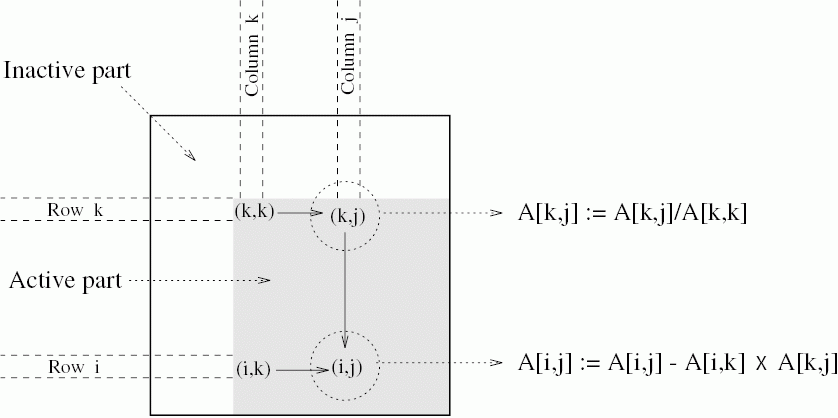
\includegraphics[width=1\textwidth]{gauss.png}
  \caption{高斯消去法示意图}
  \label{gauss}
\end{figure}
\begin{breakablealgorithm}
  \caption{普通高斯消元算法伪代码}
  \begin{algorithmic}[1] %每行显示行号  
    \Function {LU}{}
    \For {$k:=0$\ \textbf{to}\ $n$}
    \For {$j:=k+1$\ \textbf{to}\ $n$}
    \State {$A[k,j]:=A[k,j]/A[k,k]$}
    \EndFor
    \State{$A[k,k]:=1.0$}
    \For {$i:=k+1$\ \textbf{to}\ $n$}
    \For {$j:=k+1$\ \textbf{to}\ $n$}
    \State {$A[i,j]:=A[i,j]-A[i,k]*A[k,j]$}
    \EndFor
    \State{$A[i,k]:=0$}
    \EndFor
    \EndFor
    \EndFunction
  \end{algorithmic}
\end{breakablealgorithm}

观察高斯消去算法,注意到伪代码第 4,5 行第一个内嵌循环中的$A[k, j] := A[k, j]/A[k, k]$以及伪代码第$8,9,10$行双层$for$循环中的$A[i, j] := A[i, j] − A[i, k]×A[k, j]$都是可以进行向量化的循环。可以通过 OpenMP 以及 SIMD 扩展指令对这两步进行并行优化。

\section{OpenMP 算法设计}

源码链接:
\url{https://github.com/ArcanusNEO/Parallel-Programming/tree/master/5}

\subsection{测试用例的确定}

由于测试数据集较大,不便于各个平台同步,所以采用固定随机数种子为 $12345687$ 的 mt19937随机数生成器。
经过实验发现不同规模下,所有元素独立生成,限制大小在 $[0, 100]$,能够生成可以被正确消元的矩阵。

代码如下:

\begin{lstlisting}[title=测试数据集生成器,frame=trbl,language={C++}]
  uniform_real_distribution<float> dist(0, 100);
  mt19937       mt(12345687);
  int           n;
  istringstream iss(argv[1]);
  iss >> n;
  cout << n << endl;
  for (int i = 1; i <= n; ++i)
    for (int j = 1; j <= n; ++j) cout << dist(mt) << " \n"[j == n];
\end{lstlisting}

\subsection{实验环境和相关配置}

实验在华为鲲鹏 ARM 集群平台和本地 Arch Linux x86\_64 平台完成;

华为鲲鹏 ARM 集群平台使用华为毕昇 clang++ 编译器,本地 Arch Linux x86\_64 平台使用 GNU GCC 编译器;

使用 cmake 构建项目,编译开关如下:

\begin{minted}[mathescape,
  linenos,
  numbersep=5pt,
  gobble=2,
  frame=lines,
  framesep=2mm,
  highlightcolor=green!40]{cmake}
  set(CMAKE_CXX_FLAGS_RELEASE "-O3")
  set(THREADS_PREFER_PTHREAD_FLAG ON)
  find_package(OpenMP REQUIRED)
\end{minted}

实验测试了 4、8、16 线程并行的运行数据。

\subsection{算法设计}

\subsubsection{默认平凡算法}

使用一维数组模拟矩阵,避免改变矩阵大小时第二维不方便调整、必须设成最大值的问题,可以减少 cache 失效;

使用 $\#define\ matrix(i, j)\ arr[(i) * n + (j)]$ 宏,增强可读性;

\begin{lstlisting}[title=平凡算法,frame=trbl,language={C++}]
#define matrix(i, j) arr[(i) * n + (j)]
void func(int& ans, float arr[], int n) {
  for (int k = 0; k < n; ++k) {
    for (int j = k + 1; j < n; ++j) matrix(k, j) = matrix(k, j) / matrix(k, k);
    matrix(k, k) = 1.0;
    for (int i = k + 1; i < n; ++i) {
      for (int j = k + 1; j < n; ++j)
        matrix(i, j) = matrix(i, j) - matrix(i, k) * matrix(k, j);
      matrix(i, k) = 0;
    }
  }
#undef matrix
}
\end{lstlisting}

% Please add the following required packages to your document preamble:
% \usepackage{graphicx}
\begin{table}[]
  \centering
  \resizebox{\textwidth}{!}{%
    \begin{tabular}{|llll|}
      \hline
      Scale       & Reperat times & x86 ordinary (s) & arm ordinary (s) \\ \hline
      8 × 8       & 100           & 0.000001330460   & 0.000000525400   \\ \hline
      16 × 16     & 50            & 0.000001706920   & 0.000001666000   \\ \hline
      32 × 32     & 50            & 0.000003640080   & 0.000007127000   \\ \hline
      64 × 64     & 20            & 0.000015253300   & 0.000037566500   \\ \hline
      128 × 128   & 15            & 0.000098880800   & 0.000231574000   \\ \hline
      256 × 256   & 10            & 0.000716408500   & 0.001820356000   \\ \hline
      512 × 512   & 10            & 0.006722607300   & 0.014974396000   \\ \hline
      1024 × 1024 & 5             & 0.064893815400   & 0.135511226000   \\ \hline
      2048 × 2048 & 3             & 1.400074583333   & 1.101775523333   \\ \hline
      4096 × 4096 & 1             & 10.705585484000  & 13.088073440000  \\ \hline
    \end{tabular}%
  }
  \caption{所有平台平凡算法结果对比}
  \label{tab:ord}
\end{table}

\subsubsection{所有平台下只使用 OpenMP 4、8、16 线程并行化加速}

\begin{lstlisting}[title=OpenMP 并行化加速,frame=trbl,language={C++}]
  #define NUM_THREADS 8

  void func(int& ans, float arr[], int n) {
  #define matrix(i, j) arr[(i) *n + (j)]
    int   i, j, k;
    float tmp;
  #pragma omp parallel num_threads(NUM_THREADS), private(i, j, k, tmp)
    for (k = 0; k < n; ++k) {
      tmp = matrix(k, k);
  #pragma omp for
      for (j = k + 1; j < n; ++j) matrix(k, j) = matrix(k, j) / tmp;
      matrix(k, k) = 1.0;
  #pragma omp for
      for (i = k + 1; i < n; ++i) {
        tmp = matrix(i, k);
        for (j = k + 1; j < n; ++j)
          matrix(i, j) = matrix(i, j) - tmp * matrix(k, j);
        matrix(i, k) = 0;
      }
    }
  #undef matrix
  }
\end{lstlisting}

其中修改 NUM\_THREADS 宏定义可以指定不同的并行线程数。

测试了 4、8、16 的数据。

% Please add the following required packages to your document preamble:
% \usepackage{graphicx}
\begin{table}[]
  \centering
  \resizebox{\textwidth}{!}{%
    \begin{tabular}{|llllllll|}
      \hline
      Scale       & Reperat times & x86 OpenMP 4 threads (s) & x86 OpenMP 8 threads (s) & x86 OpenMP 16 threads (s) & arm OpenMP 4 threads (s) & arm OpenMP 8 threads (s) & arm OpenMP 16 threads (s) \\ \hline
      8 × 8       & 100           & 0.000007841100           & 0.000011223470           & 0.000016886970            & 0.000092409600           & 0.000126543900           & 0.000168758200            \\ \hline
      16 × 16     & 50            & 0.000016620760           & 0.000019207720           & 0.000048819040            & 0.000179391200           & 0.000235206200           & 0.000287643600            \\ \hline
      32 × 32     & 50            & 0.000029769140           & 0.000038458880           & 0.000097313150            & 0.000357201000           & 0.000496609800           & 0.000712039600            \\ \hline
      64 × 64     & 20            & 0.000063419300           & 0.000077604000           & 0.000145570260            & 0.000716369500           & 0.000993004500           & 0.001336811000            \\ \hline
      128 × 128   & 15            & 0.000164951200           & 0.000178723933           & 0.000232990467            & 0.001481558000           & 0.001898954667           & 0.002348973333            \\ \hline
      256 × 256   & 10            & 0.000460212000           & 0.000523160100           & 0.001742868100            & 0.003256248000           & 0.004177293000           & 0.005598914000            \\ \hline
      512 × 512   & 10            & 0.001627336600           & 0.001560966700           & 0.051130604200            & 0.009262748000           & 0.009874281000           & 0.011944158000            \\ \hline
      1024 × 1024 & 5             & 0.012059842800           & 0.012384870200           & 0.743364184400            & 0.045375618000           & 0.031736468000           & 0.028419450000            \\ \hline
      2048 × 2048 & 3             & 1.195753347667           & 0.823777882667           & 2.923949854667            & 0.334706430000           & 0.275254946667           & 0.112933620000            \\ \hline
      4096 × 4096 & 1             & 11.418539925000          & 9.865224839000           & 11.725731761000           & 6.097139010000           & 3.971935890000           & 2.177672700000            \\ \hline
    \end{tabular}%
  }
  \caption{所有平台 OpenMP only 结果对比}
  \label{tab:openmp}
\end{table}

\subsubsection{使用 OpenMP 及 SIMD 在 x86 平台 4、8 线程并行化加速}

\begin{lstlisting}[title=x86 OpenMP + AVX 并行化加速,frame=trbl,language={C++}]
  #define NUM_THREADS 8

  void func(int& ans, float arr[], int n) {
  #define matrix(i, j)  arr[(i) *n + (j)]
  #define pmatrix(i, j) (arr + (i * n + j))
    int    i, j, k;
    float  tmp;
    __m256 vaik, vakj, vaij, vx;
  #pragma omp parallel num_threads(NUM_THREADS), \
    private(i, j, k, tmp, vaik, vakj, vaij, vx)
    for (k = 0; k < n; ++k) {
      tmp = matrix(k, k);
  #pragma omp for
      for (j = k + 1; j < n; ++j) matrix(k, j) = matrix(k, j) / tmp;
      matrix(k, k) = 1.0;
  #pragma omp for
      for (i = k + 1; i < n; ++i) {
        vaik =
          _mm256_set_ps(matrix(i, k), matrix(i, k), matrix(i, k), matrix(i, k),
                        matrix(i, k), matrix(i, k), matrix(i, k), matrix(i, k));
        for (j = k + 1; j + 8 <= n; j += 8) {
          vakj = _mm256_loadu_ps(pmatrix(k, j));
          vaij = _mm256_loadu_ps(pmatrix(i, j));
          vx   = _mm256_mul_ps(vakj, vaik);
          vaij = _mm256_sub_ps(vaij, vx);
          _mm256_storeu_ps(pmatrix(i, j), vaij);
        }
        tmp = matrix(i, k);
        for (; j < n; ++j) matrix(i, j) = matrix(i, j) - tmp * matrix(k, j);
        matrix(i, k) = 0;
      }
    }
  #undef matrix
  }
\end{lstlisting}

% Please add the following required packages to your document preamble:
% \usepackage{graphicx}
\begin{table}[]
  \centering
  \resizebox{\textwidth}{!}{%
    \begin{tabular}{|llll|}
      \hline
      Scale       & Reperat times & x86 OpenMP 4 threads AVX (s) & x86 OpenMP 8 threads AVX (s) \\ \hline
      8 × 8       & 100           & 0.000009138760               & 0.000011101290               \\ \hline
      16 × 16     & 50            & 0.000015564840               & 0.000018825000               \\ \hline
      32 × 32     & 50            & 0.000030945160               & 0.000039081760               \\ \hline
      64 × 64     & 20            & 0.000067078900               & 0.000079877600               \\ \hline
      128 × 128   & 15            & 0.000156863733               & 0.000172293600               \\ \hline
      256 × 256   & 10            & 0.000542010200               & 0.000501830600               \\ \hline
      512 × 512   & 10            & 0.001857792100               & 0.001428114600               \\ \hline
      1024 × 1024 & 5             & 0.015659546200               & 0.011327669000               \\ \hline
      2048 × 2048 & 3             & 1.033535896333               & 0.737357611000               \\ \hline
      4096 × 4096 & 1             & 10.552043834000              & 10.662585467000              \\ \hline
    \end{tabular}%
  }
  \caption{x86 平台 OpenMP + AVX 结果对比}
  \label{tab:openmpavx}
\end{table}

\subsubsection{使用 OpenMP 及 SIMD 在 arm 平台 4、8 线程并行化加速}

\begin{lstlisting}[title=arm OpenMP + NEON 并行化加速,frame=trbl,language={C++}]
  #define NUM_THREADS 8

  void func(int& ans, float arr[], int n) {
  #define matrix(i, j)  arr[(i) *n + (j)]
  #define pmatrix(i, j) (arr + (i * n + j))
    int         i, j, k;
    float       tmp;
    float32x4_t vaik, vakj, vaij, vx;
  #pragma omp parallel num_threads(NUM_THREADS), \
    private(i, j, k, tmp, vaik, vakj, vaij, vx)
    for (k = 0; k < n; ++k) {
      tmp = matrix(k, k);
  #pragma omp for
      for (j = k + 1; j < n; ++j) matrix(k, j) = matrix(k, j) / tmp;
      matrix(k, k) = 1.0;
  #pragma omp for
      for (i = k + 1; i < n; ++i) {
        vaik = vdupq_n_f32(matrix(i, k));
        for (j = k + 1; j + 4 <= n; j += 4) {
          vakj = vld1q_f32(pmatrix(k, j));
          vaij = vld1q_f32(pmatrix(i, j));
          vx   = vmulq_f32(vakj, vaik);
          vaij = vsubq_f32(vaij, vx);
          vst1q_f32(pmatrix(i, j), vaij);
        }
        tmp = matrix(i, k);
        for (; j < n; ++j) matrix(i, j) = matrix(i, j) - tmp * matrix(k, j);
        matrix(i, k) = 0;
      }
    }
  #undef matrix
}
\end{lstlisting}

% Please add the following required packages to your document preamble:
% \usepackage{graphicx}
\begin{table}[]
  \centering
  \resizebox{\textwidth}{!}{%
    \begin{tabular}{|llll|}
      \hline
      Scale       & Reperat times & arm OpenMP 4 threads NEON (s) & arm OpenMP 8 threads NEON (s) \\ \hline
      8 × 8       & 100           & 0.000096044400                & 0.000150384800                \\ \hline
      16 × 16     & 50            & 0.000188844800                & 0.000279533400                \\ \hline
      32 × 32     & 50            & 0.000385884200                & 0.000604768200                \\ \hline
      64 × 64     & 20            & 0.000774845500                & 0.001232058000                \\ \hline
      128 × 128   & 15            & 0.001617558000                & 0.002336769333                \\ \hline
      256 × 256   & 10            & 0.003750217000                & 0.005148563000                \\ \hline
      512 × 512   & 10            & 0.011932396000                & 0.012737347000                \\ \hline
      1024 × 1024 & 5             & 0.062839944000                & 0.043704944000                \\ \hline
      2048 × 2048 & 3             & 0.504436153333                & 0.303472556667                \\ \hline
      4096 × 4096 & 1             & 7.025737910000                & 4.243570140000                \\ \hline
    \end{tabular}%
  }
  \caption{arm 平台 OpenMP + NEON 结果对比}
  \label{tab:openmpneon}
\end{table}

\section{实验结果分析}

观察比较表 \ref{tab:ord}、\ref{tab:dynamic}、\ref{tab:sem}、\ref{tab:sem-all}、\ref{tab:barrier}
可以发现使用线程池加信号量或者栅栏同步多线程的方式,在 arm 平台可以大幅提升性能,小数据量下效果微弱甚至不如平凡算法,但是大数据量有成倍提升。

4096 × 4096 数据规模 arm 平台下普通信号量同步用时 5.892652880000 s,平凡算法用时 13.088073440000 s,加速比 2.221083391;
所有循环纳入线程回调函数用时 5.209506790000 s,加速比 2.51234406;
使用栅栏同步可以继续获得性能提升,用时 5.017878950000 s,加速比 2.608287998;
使用栅栏同步加上 NEON 指令集 SIMD 优化可以继续获得性能提升,用时 4.582658000000 s,加速比 2.856000478;

然而,使用动态线程的方式处理会导致性能倒退,不如平凡算法:可以发现创建线程和销毁线程的开销巨大,造成性能下降。

比较表 \ref{tab:ord} 两平台的平凡算法,可以发现本地 x86 平台单核性能领先于 arm 平台;但是比较表 \ref{tab:sem}、\ref{tab:sem-all}、\ref{tab:barrier} 中两平台可以发现,对于小数据量还是 x86 平台领先,但是 arm 平台在 大数据量下表现更优,实现反超。
在 x86 平台上使用信号量同步并将所有循环纳入线程回调函数或者栅栏同步时无助于性能提升。

% Please add the following required packages to your document preamble:
% \usepackage{graphicx}
\begin{table}[]
  \centering
  \resizebox{\textwidth}{!}{%
    \begin{tabular}{|lllllll|}
      \hline
      Scale       & Reperat times & x86 ordinary (s) & x86 dynamic (s)  & x86 semaphore (s) & x86 semaphore all (s) & x86 barrier (s) \\ \hline
      8 × 8       & 100           & 0.000001330460   & 0.000408343660   & 0.000220605390    & 0.000295141480        & 0.000356697420  \\ \hline
      16 × 16     & 50            & 0.000001706920   & 0.001760123900   & 0.000319653680    & 0.000439524060        & 0.000631893380  \\ \hline
      32 × 32     & 50            & 0.000003640080   & 0.007970805160   & 0.000513098020    & 0.000699135760        & 0.000695531360  \\ \hline
      64 × 64     & 20            & 0.000015253300   & 0.031911559450   & 0.000966301100    & 0.001294170900        & 0.001590516150  \\ \hline
      128 × 128   & 15            & 0.000098880800   & 0.130038008533   & 0.001879047067    & 0.002380586333        & 0.003217344067  \\ \hline
      256 × 256   & 10            & 0.000716408500   & 0.515502232000   & 0.003608040400    & 0.005267385000        & 0.004891007500  \\ \hline
      512 × 512   & 10            & 0.006722607300   & 2.105457739200   & 0.011124012800    & 0.013941518400        & 0.013557604400  \\ \hline
      1024 × 1024 & 5             & 0.064893815400   & 8.558513793600   & 0.050837437000    & 0.065091814800        & 0.055628581000  \\ \hline
      2048 × 2048 & 3             & 1.400074583333   & 33.120794944000  & 1.160066842000    & 1.268976019000        & 1.297545969000  \\ \hline
      4096 × 4096 & 1             & 10.705585484000  & 139.134070615000 & 11.558711337000   & 11.411054368000       & 12.573134918000 \\ \hline
    \end{tabular}%
  }
  \caption{x86 平台所有结果对比}
  \label{tab:x86}
\end{table}

% Please add the following required packages to your document preamble:
% \usepackage{graphicx}
\begin{table}[]
  \centering
  \resizebox{\textwidth}{!}{%
    \begin{tabular}{|llllllll|}
      \hline
      Scale       & Reperat times & arm ordinary (s) & arm dynamic (s)  & arm semaphore (s) & arm semaphore all (s) & arm barrier (s) & arm barrier with neon (s) \\ \hline
      8 × 8       & 100           & 0.000000525400   & 0.001069426000   & 0.000414891100    & 0.000451200400        & 0.000430526600  & 0.000414370700            \\ \hline
      16 × 16     & 50            & 0.000001666000   & 0.004892212000   & 0.000546852800    & 0.000708521400        & 0.000631723800  & 0.000546980800            \\ \hline
      32 × 32     & 50            & 0.000007127000   & 0.020191436600   & 0.000823440200    & 0.001197251400        & 0.000821696600  & 0.000801270200            \\ \hline
      64 × 64     & 20            & 0.000037566500   & 0.080842077000   & 0.001490467500    & 0.001791016000        & 0.001415785500  & 0.001367928500            \\ \hline
      128 × 128   & 15            & 0.000231574000   & 0.338396283333   & 0.002734098000    & 0.004017182667        & 0.003097213333  & 0.002935288000            \\ \hline
      256 × 256   & 10            & 0.001820356000   & 1.318216261000   & 0.005964593000    & 0.009138907000        & 0.005816473000  & 0.005479598000            \\ \hline
      512 × 512   & 10            & 0.014974396000   & 5.282467893000   & 0.018504859000    & 0.020430503000        & 0.017091460000  & 0.015217643000            \\ \hline
      1024 × 1024 & 5             & 0.135511226000   & 21.790754608000  & 0.077263730000    & 0.088223814000        & 0.082351834000  & 0.080288012000            \\ \hline
      2048 × 2048 & 3             & 1.101775523333   & 85.470935310000  & 0.541380500000    & 0.604317156667        & 0.503372826667  & 0.455167490000            \\ \hline
      4096 × 4096 & 1             & 13.088073440000  & 353.288384510000 & 5.892652880000    & 5.209506790000        & 5.017878950000  & 4.582658000000            \\ \hline
    \end{tabular}%
  }
  \caption{arm 平台所有结果对比}
  \label{tab:arm}
\end{table}

\begin{figure}[h]
  \centering
  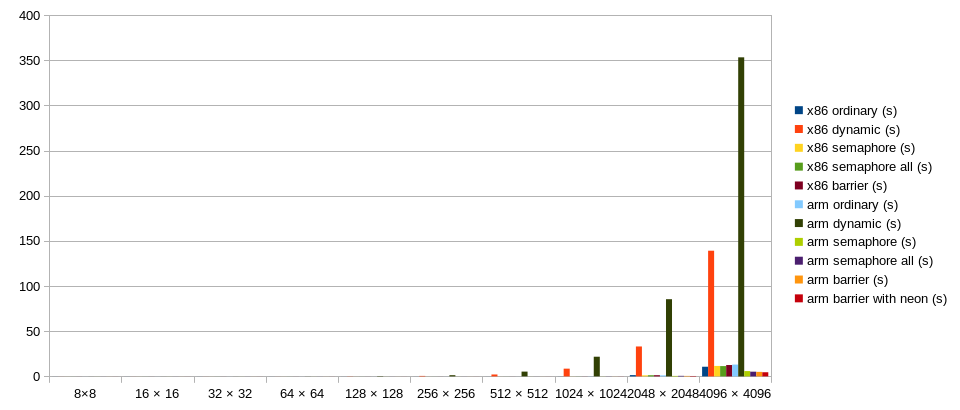
\includegraphics[width=\textwidth]{all.png}
  \caption{所有平台所有结果对比柱状图}
  \label{pic:all}
\end{figure}

\begin{figure}[h]
  \centering
  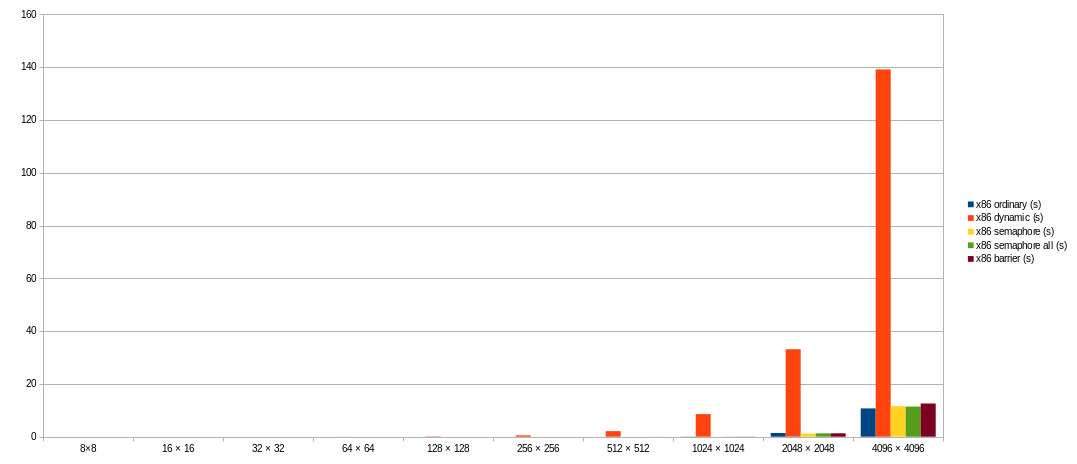
\includegraphics[width=\textwidth]{x86.png}
  \caption{x86 平台所有结果对比柱状图}
  \label{pic:x86}
\end{figure}

\begin{figure}[h]
  \centering
  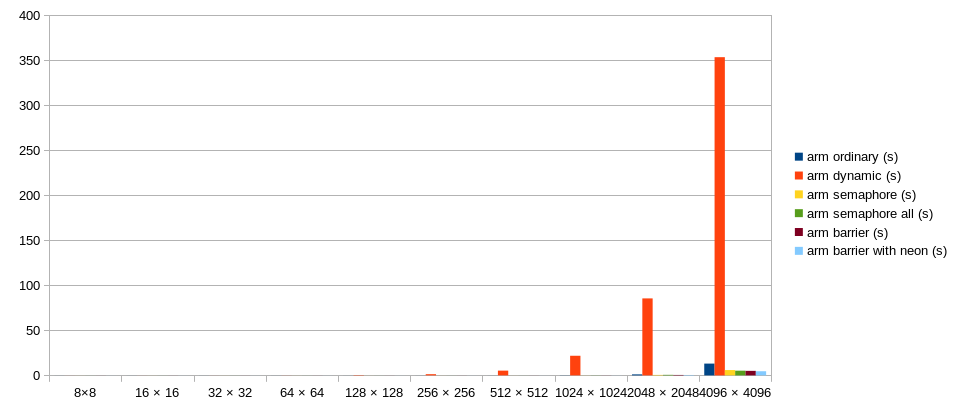
\includegraphics[width=\textwidth]{arm.png}
  \caption{arm 平台所有结果对比柱状图}
  \label{pic:arm}
\end{figure}

\begin{figure}[h]
  \centering
  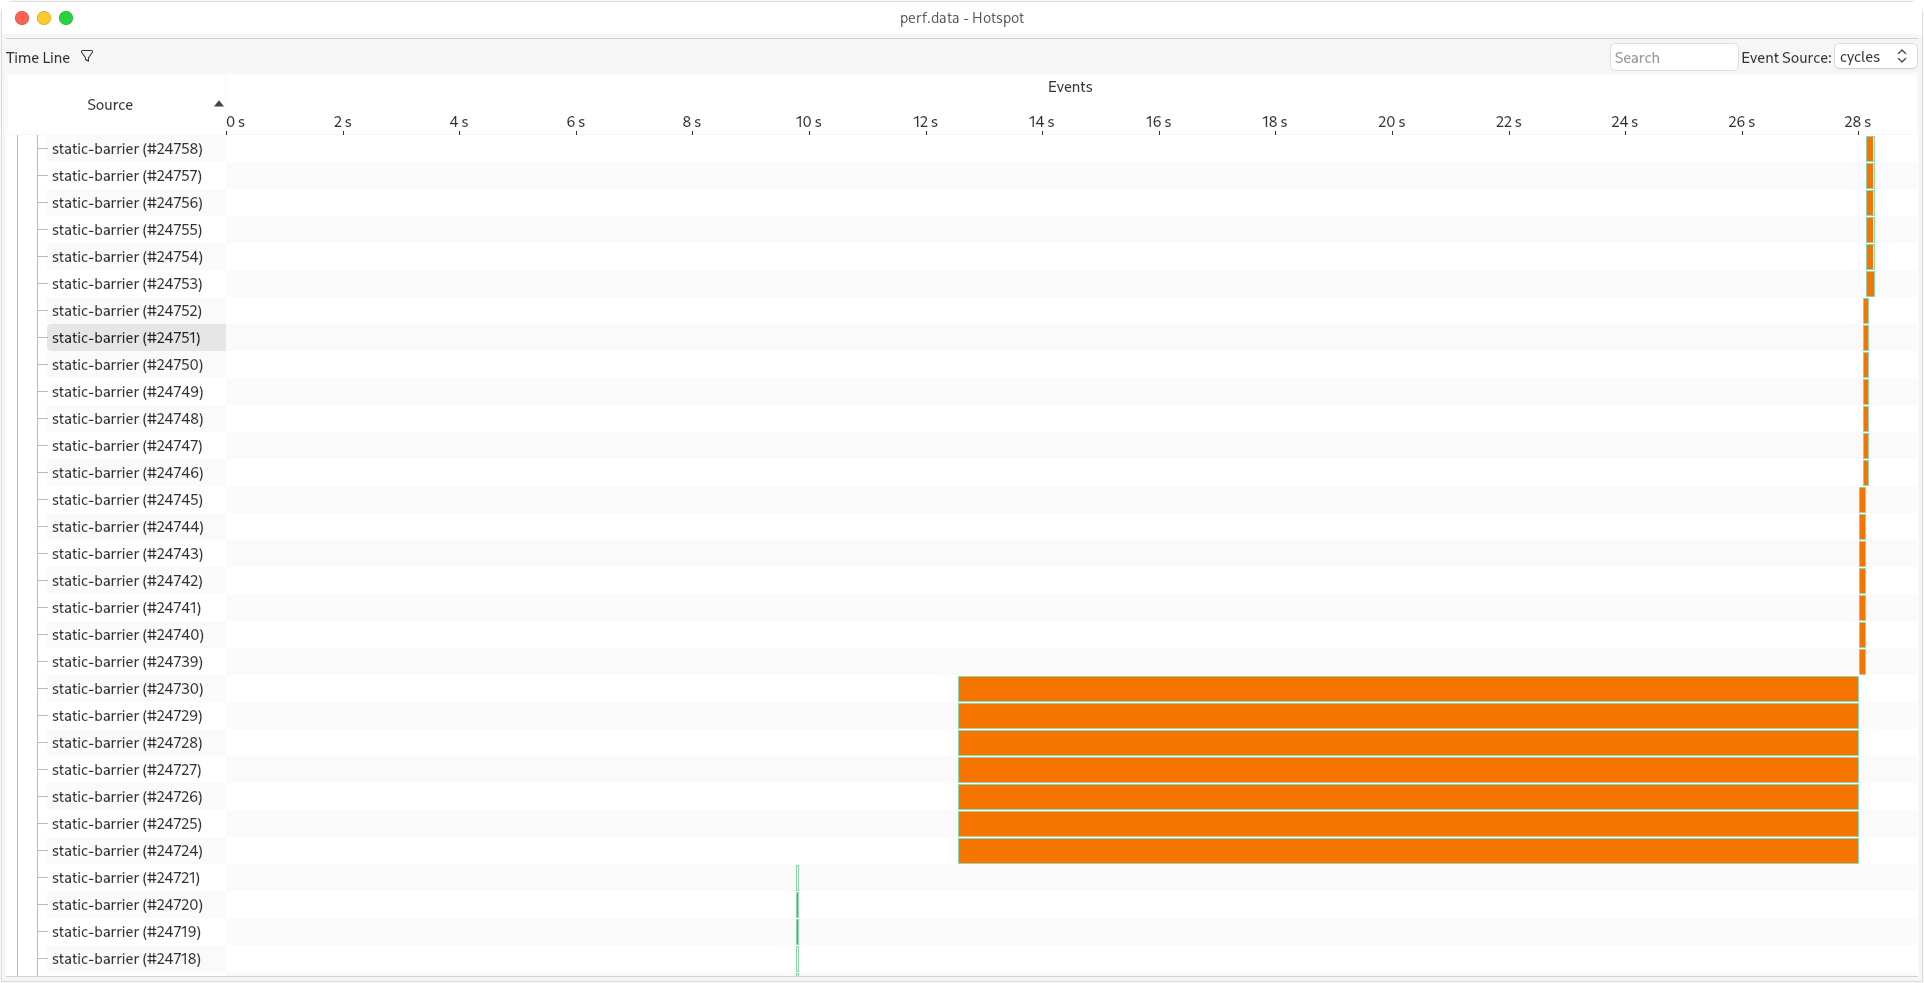
\includegraphics[width=\textwidth]{barrier-perf.png}
  \caption{对 barrier 使用 perf 分析}
  \label{pic:perf}
\end{figure}

如图 \ref{pic:perf},对 barrier 使用 perf 进行分析可以发现并行度良好。

% \newpage

% \section{参考文献}
% \cite{1}\cite{2}\cite{3}\cite{4}\cite{5}\cite{6}

% \bibliographystyle{plain}
% \bibliography{Parallel-Programming-0.bib}

\end{document}